\documentclass{beamer}

\usepackage{beamerthemesplit}
\usepackage{graphicx} % Required to insert images
\usepackage[utf8]{inputenc}
\usepackage[T1]{fontenc}
\usepackage{lmodern}
\usepackage{verbatim}

\title{Dominion Datamining}
\author{Khaoula TAGNAOUTI, Liliana LOPEZ, Willian VER VALEM, Elmer BAYOL}

\begin{document}
\maketitle

\begin{frame}
  \frametitle{Introduction}
  test phrase
  \begin{itemize}
    \item Serveur ouvert de 2010 à 2013
    \item 12 Millions de parties enrigistrées
    \item Wiki regroupant des informations sur les stratégies
  \end{itemize}

\end{frame}

\begin{frame}
  \frametitle{Introduction}
  \framesubtitle{Travail demandé}
  \begin{itemize}
    \item 
  \end{itemize}
\end{frame}
  
\begin{frame}
  \frametitle{Fonctionnalités}
  \begin{itemize}
  \item Parser
  \item Stockage des données
  \item calcul d'elo
  \end{itemize}
\end{frame}

\begin{frame}
  \frametitle{Fonctionnalités}
  \framesubtitle{Parser}
  \begin{itemize}
  \item 99.8\% des logs sont parsés
  \item Seul le header est parsé
  \item Est capable de travailler avec les logs compressés
  \end{itemize}
\end{frame}

\begin{frame}
  \frametitle{Fonctionnalités}
  \framesubtitle{Stockage des données}
  \begin{itemize}
  \item Stockage des parties
  \item Stockage d'elo global pour chaque joueur
  \item Stockage de liste des parties d'un joueur
  \end{itemize}
\end{frame}

\begin{frame}
  \frametitle{Fonctionnalités}
  \framesubtitle{Calcul d'elo}
  \begin{itemize}
  \item Chaque partie est prise en ordre chronologique
  \item Prise en compte de l'elo global
  \item Mise a jour du nouvel elo global du joueur
  \item Ajout de l'elo du joueur au moment de la partie (ne varie pas)
  \end{itemize}
\end{frame}

\begin{frame}
  \frametitle{Fonctionnalités}
  \framesubtitle{Calcul d'elo}
  \begin{center}
    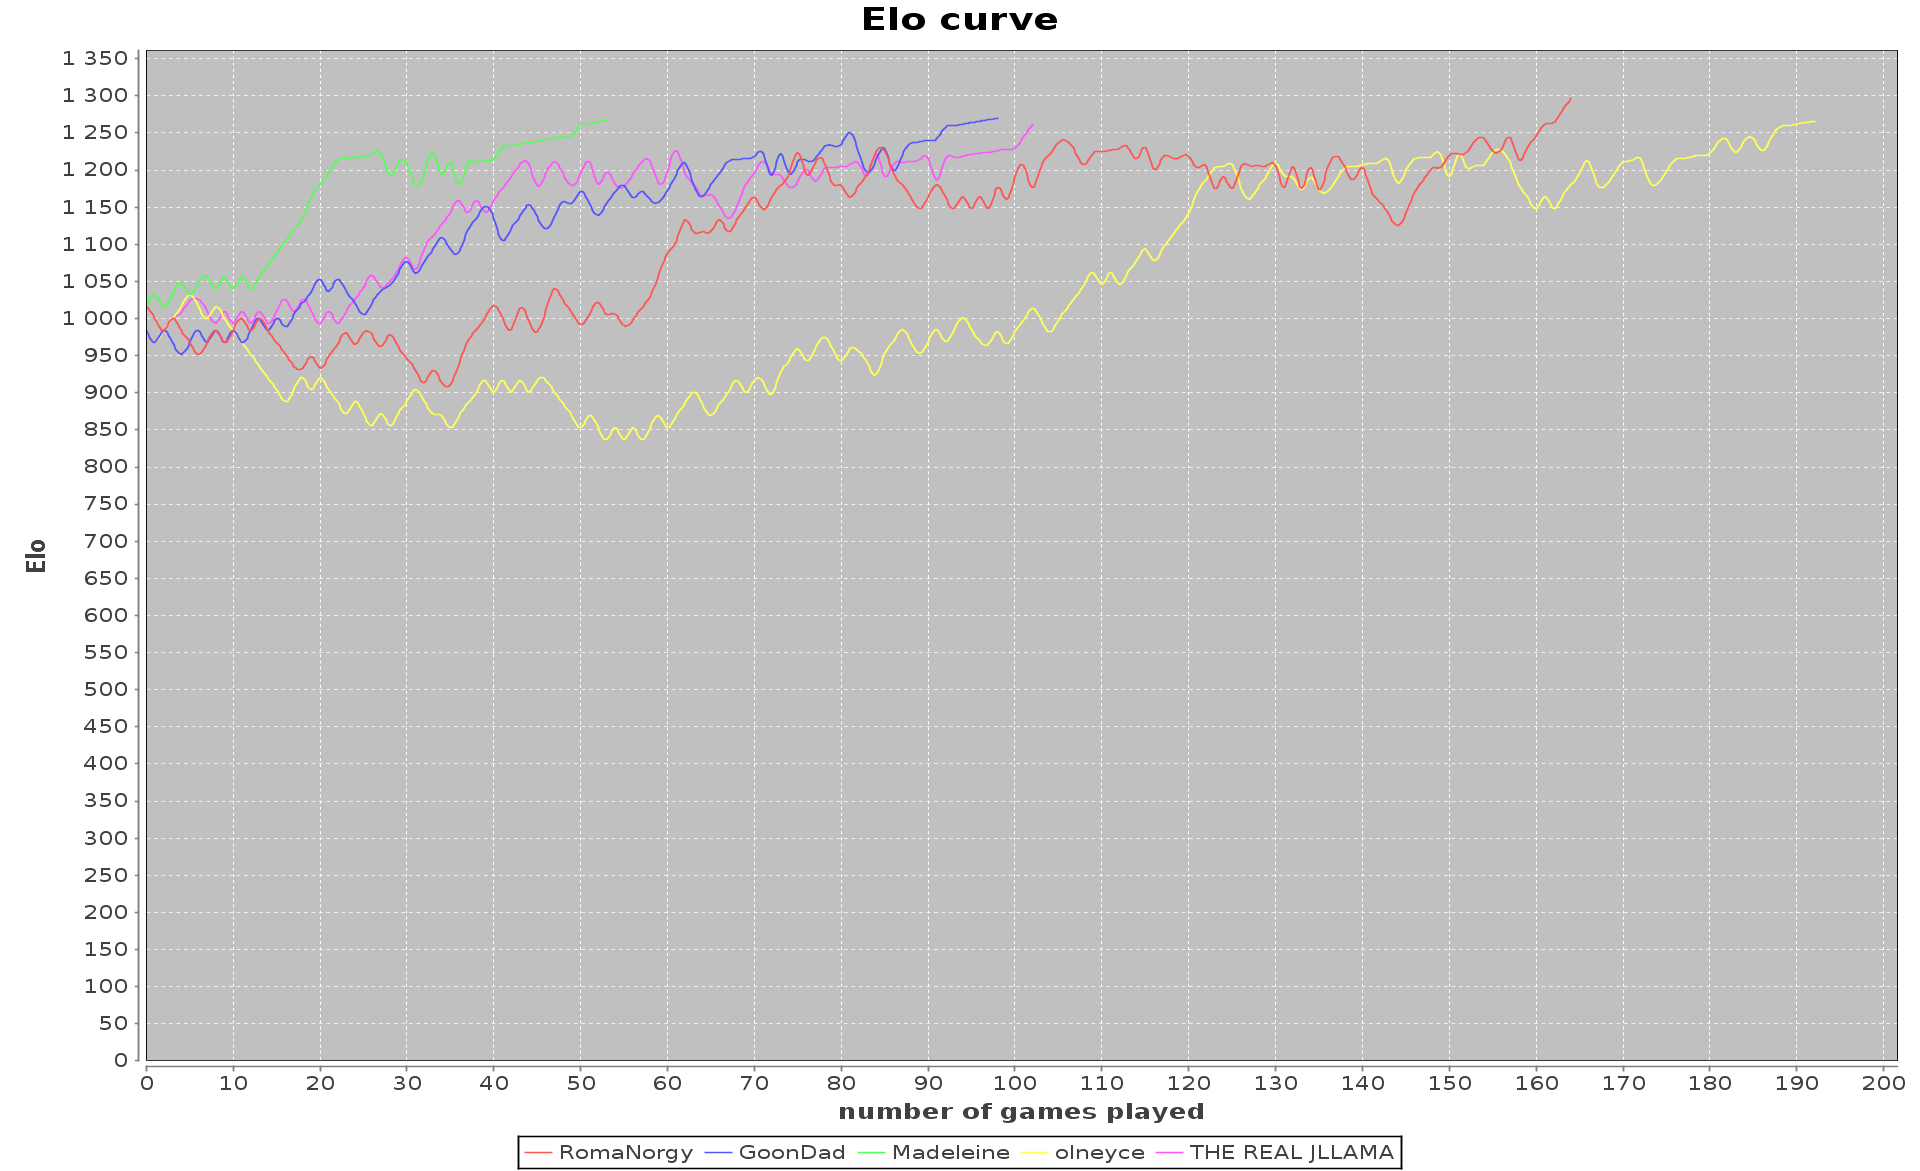
\includegraphics[scale=0.15,keepaspectratio]{elo}
  \end{center}
\end{frame}

\begin{frame}
  \frametitle{Architecture}
  \begin{center}
    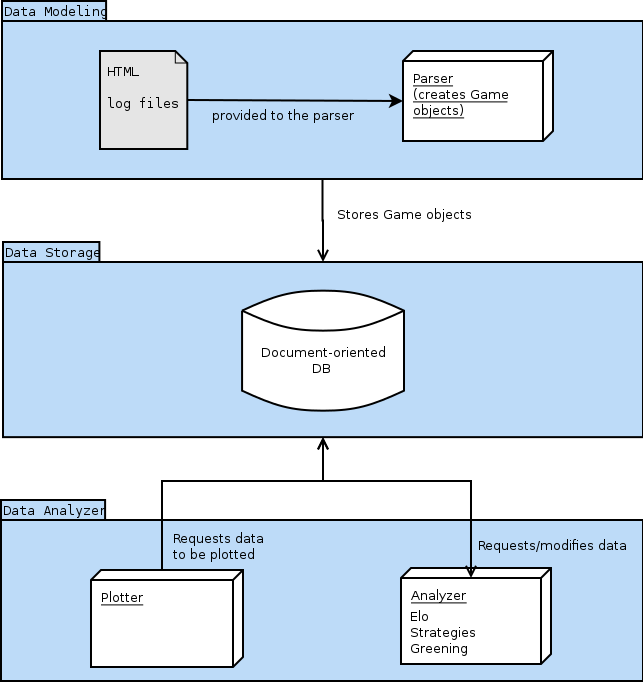
\includegraphics[scale=0.30,keepaspectratio]{globalArch_v2}
    \end{center}
\end{frame}

\begin{frame}
  \frametitle{Architecture}
  \begin{center}
    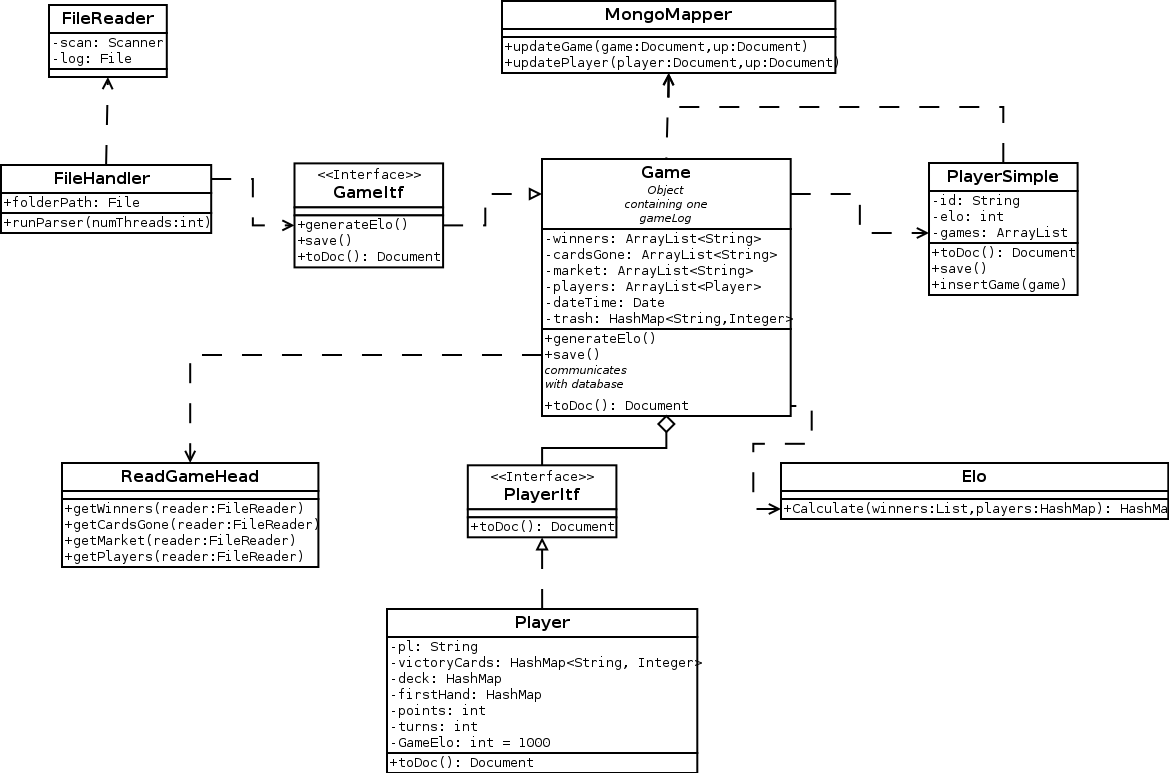
\includegraphics[scale=0.27,keepaspectratio]{parserArch}
    \end{center}
\end{frame}

\begin{frame}
  \frametitle{Aspects techniques}
…
\end{frame}

\end{document}
